%%% TOCL
%%% Version 1
% TOCL enhances the Object Constraint Language (OCL) by enabling the 
% specification of properties that must hold over time, across multiple states of 
% a system. While standard OCL is limited to evaluating constraints within a 
% single system state or across a single state transition (via pre- and postconditions), 
% many system requirements involve dynamic behaviors that unfold over sequences of states. 
% Examples include properties such as "eventually, the system will reach a stable state" 
% or "once a condition is met, it must remain true thereafter." To address this, 
% TOCL, as introduced by Ziemann and Gogolla \cite{TOCL}, extends OCL with 
% elements of linear temporal logic, allowing these temporal properties to be expressed 
% directly within a familiar OCL-like syntax.

% TOCL introduces a comprehensive set of temporal operators, divided into future 
% and past categories, which are adopted in TOCL+ as the foundation for temporal 
% reasoning. Below, we review these operators, their syntax, semantics, and provide 
% illustrative examples.

%%% Version 1
% These operators enable precise specification of temporal relationships, making TOCL suitable for modeling and verifying dynamic system behaviors.

%%% Sample
% Future Operators:

% next e: True if the expression e holds in the next state.
% always e: True if e holds in the current state and all subsequent states.
% sometime e: True if e holds in the current state or at least one future state.
% always e1 until e2: True if e1 remains true until e2 becomes true, or if e1 remains true indefinitely if e2 never becomes true.
% sometime e1 before e2: True if e1 becomes true at some point before e2 does, or if e1 becomes true and e2 never does.

% Past Operators:

% previous e: True if e was true in the previous state (or if there is no previous state, i.e., at the initial state).
% alwaysPast e: True if e was true in all past states.
% sometimePast e: True if e was true in at least one past state.
% always e1 since e2: True if e1 has been true since the last time e2 was true.
% sometime e1 since e2: True if e1 has been true at some point since the last time e2 was true.

%
% \subsubsection{Syntax and Semantics}
% The original syntax of TOCL in [29] was defined using mathematical notations as opposed to EBNF.
% author = {Lail, Mustafa Al and Rosales, Antonio and Cardenas, Hector and Hamann, Lars and Perez, Alfredo},
% created EBNF grammar of TOCL in \cite{TOCL2OCL}. We also adopted this EBNF grammar to define the syntax of TOCL in our work.
% The syntax of TOCL integrates these temporal operators seamlessly into OCL expressions, allowing them to be used within invariants, preconditions, and postconditions. For example:

% An invariant using \textit{always} operator:
% \begin{lstlisting}[style=toclstyle]
% context C inv: always (self.attribute > 0)
% \end{lstlisting}
% context C inv:
%   always (self.attribute > 0)

% A condition using \textit{next} operator:
% \begin{lstlisting}[style=toclstyle]
% context C inv:
%   self.state = #active implies next (self.state = #idle)
% \end{lstlisting}

% The semantics of these operators are defined over sequences of system states, with 
% formal definitions provided by Ziemann and Gogolla \cite{TOCL} based on state 
% sequences ($\hat{\sigma} = \langle \sigma_0, \sigma_1, \ldots \rangle$). For the 
% complete formal treatment, readers are referred to the original research.

% The semantics of these operators are defined over infinite sequences of system states, where each state represents a snapshot of the system at a given time. 
% Formal definitions of the semantics are provided in [28], based on a state sequence ($\hat{\sigma} = \langle \sigma_0, \sigma_1, \ldots \rangle$), ensuring a rigorous foundation for TOCL. For a detailed formal treatment, readers are referred to the original paper.
% The evaluation of an expression depends on its position within this sequence:

% \begin{itemize}
%   \item \textbf{next $e$:} True if $e$ holds at the state immediately following the current one.
%   \item \textbf{always $e$:} True if $e$ holds at the current state and all future states.
%   \item \textbf{sometime $e$:} True if $e$ holds at the current state or some future state.
%   \item \textbf{For past operators:} The evaluation considers the sequence of states preceding the current state, with \textit{previous $e$} being true if $e$ held in the prior state, and so forth.
% \end{itemize}
% next e is true if e holds at the state immediately following the current one.
% always e is true if e holds at the current state and all future states.
% sometime e is true if e holds at the current state or some future state.
% For past operators, the evaluation considers the sequence of states preceding the current state, with previous e being true if e held in the prior state, and so forth.

%%% Event extension


%%% VERSION 2
%%%%% Refactoring
% TOCL (Temporal OCL), introduced by Ziemann and Gogolla \cite{TOCL}, extends OCL with temporal operators for specifying properties that must hold across multiple system states. It incorporates elements of linear temporal logic while maintaining OCL's familiar syntax, enabling developers to express temporal constraints directly within their models. TOCL extends standard OCL with a comprehensive set of temporal operators categorized into future operators (next, always, sometime, until, before) and past operators (previous, alwaysPast, sometimePast, since), each with well-defined semantics for reasoning about system behavior over time. These operators follow the principles of linear temporal logic but are adapted to work within OCL's object-oriented context, preserving OCL's typing system and navigation capabilities. By integrating temporal reasoning directly into OCL, TOCL provides a unified formalism that addresses the fundamental limitations of standard OCL when specifying dynamic system aspects, particularly those involving sequences of states or temporal relationships between conditions.

% In this thesis, we leverage TOCL, as introduced by Ziemann and Gogolla \cite{TOCL}, 
% as the temporal foundation for specifying properties that must hold over time across 
% multiple states of a system. Standard Object Constraint Language (OCL) is limited to 
% evaluating constraints within a single system state or across a single state transition 
% (via pre- and postconditions), which is insufficient for capturing the dynamic behaviors 
% inherent in many system requirements. For instance, properties such as "eventually, 
% the system will reach a stable state" or "once a condition is met, it must remain 
% true thereafter" require reasoning over sequences of states. TOCL addresses this limitation 
% by extending OCL with elements of linear temporal logic, enabling the expression of such 
% temporal properties within a familiar OCL-like syntax.

% TOCL's comprehensive set of temporal operators, categorized into future and past 
% operators, provides the essential temporal reasoning capabilities for our work. 
% In this thesis, we adopt these operators unchanged as the basis for modeling and 
% verifying dynamic system behaviors over time. However, to address systems that 
% exhibit reactive behaviors driven by specific events, we extend TOCL into TOCL+ 
% by integrating novel event-based constructs. This extension, detailed in the next 
% section, complements TOCL’s temporal framework, enabling a more holistic specification 
% of both state-based temporal properties and event-driven dynamics. Below, we review 
% the adopted TOCL temporal operators, their syntax, and semantics, which serve as 
% the cornerstone of TOCL+.

%%%
% \subsubsection{Adopted TOCL Temporal Operators}
% TOCL defines two categories of temporal operators that we adopt in our work:

% \paragraph{Future Operators:}
% \begin{itemize}
%     \item \textbf{next $e$:} True if the expression $e$ holds in the next state.
%     \item \textbf{always $e$:} True if $e$ holds in the current state and all subsequent states.
%     \item \textbf{sometime $e$:} True if $e$ holds in the current state or at least one future state.
%     \item \textbf{always $e_1$ until $e_2$:} True if $e_1$ remains true until $e_2$ becomes true, or if $e_1$ remains true indefinitely if $e_2$ never becomes true.
%     \item \textbf{sometime $e_1$ before $e_2$:} True if $e_1$ becomes true at some point before $e_2$ does, or if $e_1$ becomes true and $e_2$ never does.
% \end{itemize}

% \paragraph{Past Operators:}
% \begin{itemize}
%     \item \textbf{previous $e$:} True if $e$ was true in the previous state (or if there is no previous state, i.e., at the initial state).
%     \item \textbf{alwaysPast $e$:} True if $e$ was true in all past states.
%     \item \textbf{sometimePast $e$:} True if $e$ was true in at least one past state.
%     \item \textbf{always $e_1$ since $e_2$:} True if $e_1$ has been true since the last time $e_2$ was true.
%     \item \textbf{sometime $e_1$ since $e_2$:} True if $e_1$ has been true at some point since the last time $e_2$ was true.
% \end{itemize}

% For the formal semantics of these operators, we refer to the original work by 
% Ziemann and Gogolla \cite{TOCL}, which defines them over sequences of system states.

%%%
% \subsubsection{Example Specifications}
% To demonstrate the practical application of these operators, we apply them to 
% the software system case study introduced in Chapter 1:


\subsection{Event Constructs in OCL}
% To overcome the limitations of TOCL in specifying event-based properties, we
% we propose an extension to TOCL that supports specifying events. The notion of event is
% borrowed from \cite{TemporalAndEventOCL}, which defines events as predicates that specify
% a set of instants within the time line. In section \ref{sec:ocl}, we discussed the
% different types of events in the object-oriented approach. There are operation
% (call/start/end) events, time-triggered events, and state change events. In this work,
% we focus on extending OCL with the necessary constructs for both operation and state change
% events. We also adopt the synchronous paradigm, and we merge the operation
% (call/start/end) events into one call event, named \texttt{isCalled}, that leads the
% system from a pre-state to a post-state without considering intermediate change states.

% The keyword ‘isCalled’ represents a call event, which corre
% sponds to a call to an operation. Under the hypothesis of atomicity of operations,
% we merge into a single call event, the events corresponding to the call, the start,
% and the end of an operation. A call event has one parameter, which is the operation
% being called with its parameters. The keyword ‘becomesTrue’ denotes a state change event
% parameterized with the OCL expression provided as parameter: it corresponds
% to the state in which the input expression becomes true (which implies that in
% the previous state it evaluated to false).

% \begin{itemize}
%     \item \textbf{isCalled}: A generic event construct that unifies operation events. 
%     It detects when an operation is invoked on an object, representing the atomic 
%     transition from a pre-state to a post-state. It has one required parameter, 
%     \texttt{op}, which is the operation being called with its parameters.
    
%     \item \textbf{becomesTrue}: A state change event that is parameterized by an OCL 
%     boolean expression P. It designates a step in which P becomes true (i.e., P was 
%     evaluated to false in the previous state and is true in the current state). 
% \end{itemize}

% \subsection{Event Constructs in OCL}

% \hspace{1cm} To address TOCL's limitations in expressing event-based properties, we 
% propose TOCL+, an extension that introduces explicit event specification capabilities. 
% We adopt the concept of events from \cite{TemporalAndEventOCL}, which defines events 
% as predicates identifying specific instants in time. As discussed in Section 
% \ref{sec:ocl}, object-oriented systems typically recognize multiple event types: 
% operation events (call/start/end), time-triggered events, and state change events. 
% Our extension focuses specifically on operation and state change events, as they 
% capture the fundamental interactions in object-oriented systems.

% Following the synchronous paradigm for its well-defined formal semantics, TOCL+ 
% merges operation events (call/start/end) into a single construct named 
% \texttt{isCalled}. This construct represents the atomic transition from a pre-state 
% to a post-state without intermediate states, providing a clean abstraction for 
% verification. This atomicity assumption simplifies reasoning about system behavior 
% while still capturing essential reactive properties.

% TOCL+ introduces two primary event constructs. The first construct, \textbf{isCalled}, 
% is a generic event construct that unifies operation events. It detects when an 
% operation is invoked on an object, representing the atomic transition from a 
% pre-state to a post-state. It has one required parameter, \texttt{op}, which is the 
% operation being called with its parameters.

% The second construct, \textbf{becomesTrue}, represents a state change event 
% parameterized by an OCL boolean expression P. It designates a step in which P becomes 
% true (i.e., P was evaluated to false in the previous state and is true in the current 
% state).

% Both event constructs are illustrated in Figure \ref{fig:event_constructs}.

% % Event figures
% \begin{figure}
%     \centering
%     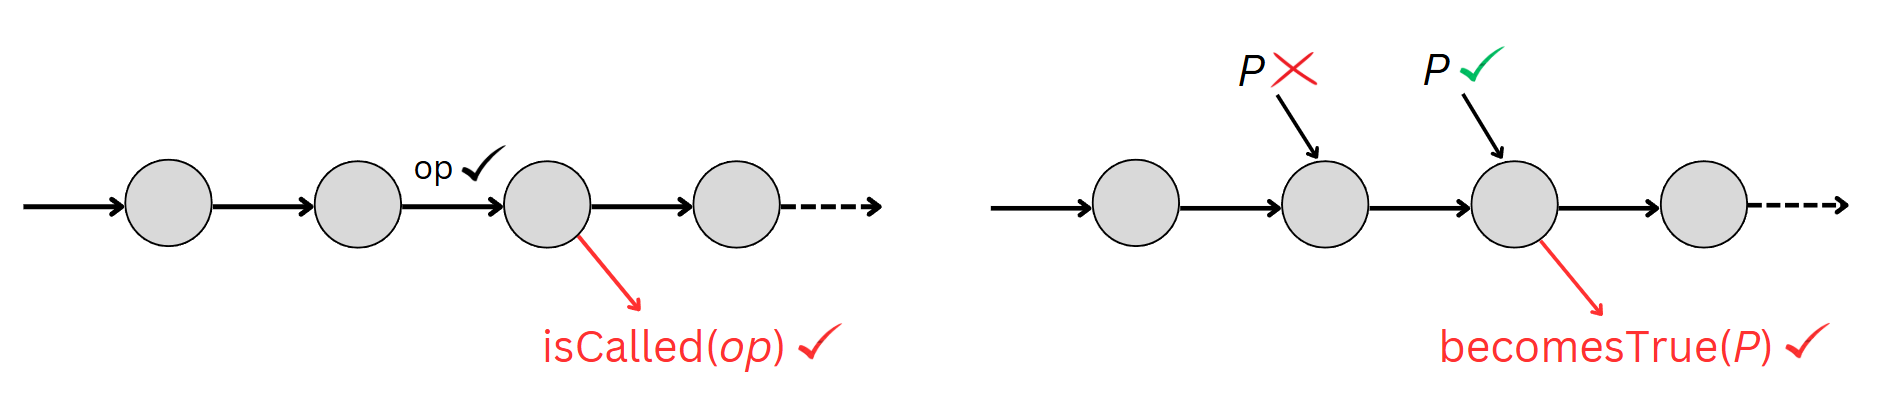
\includegraphics[width=1\textwidth]{figures/c2/events_visual.png}
%     \caption{Events.}
%     \label{fig:event_constructs}
% \end{figure}

% We also extend TOCL with bounded existence support to specify properties like
% - an event occurs k times.
% - an event occurs at least k times.
% - an event occurs at most k times.

% Back to our temporal properties \ref{fig:temporal_properties}. We can simply specify 
% them using TOCL+ in \ref{lst:tocl+}:

% \begin{lstlisting}[
%     style=toclstyle, 
%     caption={TOCL+ Specifications.}, 
%     label={lst:tocl+}
% ]
% context System
% /*
% An application loading must precede its run.
% */
% inv safety1: 
%     self.runningApps->notEmpty() implies
%     self.runningApps->forAll(app |
%         isCalled(run(app : Application)) implies
%         sometimePast isCalled(load(app : Application))
%     )

% /*
% There must be an install operation between an application's loading and its running.
% */
% inv safety2: 
%     self.runningApps->notEmpty() implies
%     self.runningApps->forAll(app |
%         isCalled(run(app : Application)) implies (
%             sometime isCalled(install())
%             since isCalled(load(app : Application))
%         )
%     )

% /*
% Each application can be loaded at most one time.
% */
% inv safety3:
%     self.installedApps->notEmpty() implies
%     self.installedApps->forAll(app |
%         sometimePast isCalled(load(app : Application))
%         at most 1 times
%     )

% /*
% Every loaded application will eventually be installed.
% */
% inv liveness:
%     self.loadedApps->notEmpty() implies
%     self.loadedApps->forAll(app | 
%         sometime isCalled(install())
%     )
% \end{lstlisting}

% Write about the help of Event construct in specifying event-related temporal properties

% \subsection{Adopted TOCL Temporal Operators}

% \hspace{1cm} TOCL (Temporal OCL), introduced by Ziemann and Gogolla \cite{TOCL}, 
% extends OCL with temporal operators for specifying properties that must hold across 
% multiple system states. It incorporates elements of linear temporal logic while 
% maintaining OCL's familiar syntax, enabling developers to express temporal constraints 
% directly within their models. TOCL extends standard OCL with a comprehensive set of 
% temporal operators categorized into future operators (next, always, sometime, until, 
% before) and past operators (previous, alwaysPast, sometimePast, since), each with 
% well-defined semantics for reasoning about system behavior over time. These operators 
% follow the principles of linear temporal logic but are adapted to work within OCL's 
% object-oriented context, preserving OCL's typing system and navigation capabilities. 
% By integrating temporal reasoning directly into OCL, TOCL provides a unified formalism 
% that addresses the fundamental limitations of standard OCL when specifying dynamic 
% system aspects, particularly those involving sequences of states or temporal 
% relationships between conditions.

% In our work, we adopt the following temporal operators from TOCL:

% \paragraph{Future Operators:} 
% \begin{itemize} 
%     \item \textbf{next $e$:} True if the expression $e$ holds in the next state. 
%     \item \textbf{always $e$:} True if $e$ holds in the current state and all subsequent states. 
%     \item \textbf{sometime $e$:} True if $e$ holds in the current state or at least one future state. 
%     \item \textbf{always $e_1$ until $e_2$:} True if $e_1$ remains true until $e_2$ becomes true, or if $e_1$ remains true indefinitely if $e_2$ never becomes true. 
%     \item \textbf{sometime $e_1$ before $e_2$:} True if $e_1$ becomes true at some point before $e_2$ does, or if $e_1$ becomes true and $e_2$ never does. 
% \end{itemize}

% \paragraph{Past Operators:} \begin{itemize} 
%     \item \textbf{previous $e$:} True if $e$ was true in the previous state (or if there is no previous state, i.e., at the initial state). 
%     \item \textbf{alwaysPast $e$:} True if $e$ was true in all past states. 
%     \item \textbf{sometimePast $e$:} True if $e$ was true in at least one past state. 
%     \item \textbf{always $e_1$ since $e_2$:} True if $e_1$ has been true since the last time $e_2$ was true. 
%     \item \textbf{sometime $e_1$ since $e_2$:} True if $e_1$ has been true at some point since the last time $e_2$ was true. 
% \end{itemize}
% For the formal semantics of these operators, we refer to the original work by Ziemann and Gogolla \cite{TOCL}.

% To illustrate the capabilities of these operators, we will specify the temporal 
% properties of the Software System introduced in Chapter 1 (Figure \ref{fig:temporal_properties}).
% using TOCL.
% \begin{lstlisting}[
%     style=toclstyle, 
%     caption={TOCL Specification for Safety 1 and 2 property.}, 
%     label={lst:tocl_safety12}
% ]
% context System 
% /*
% An application loading must precede its run.
% */
% inv safety1: 
%     self.runningApps->notEmpty() implies 
%     self.runningApps->forAll(app | 
%         sometimePast self.loadedApps->includes(app)
%     )
% /*
% There must be an install operation between an application's loading and its running.
% */
% inv safety2: 
%     self.loadedApps->notEmpty() implies 
%     self.loadedApps->forAll(app | 
%         sometime self.installedApps->includes(app) 
%         before self.runningApps->includes(app)
%     )
% \end{lstlisting}
% As shown in Listing \ref{lst:tocl_safety12}, TOCL allows us to elegantly express 
% properties that span multiple system states. Safety 1 uses the \texttt{sometimePast} 
% operator to verify that any application in the \texttt{runningApps} collection must 
% have previously been in the \texttt{loadedApps} collection, capturing the temporal 
% ordering requirement. Safety 2 utilizes the \texttt{before} operator to specify that 
% an application must be in the \texttt{installedApps} collection before it appears 
% in the \texttt{runningApps} collection. These specifications are impossible to 
% formulate in standard OCL, which has no operators for referring to past or future 
% states beyond a single transition.

% However, TOCL still has important limitations when it comes to specifying event-based 
% properties. For Safety 3 ("Each application can be loaded at most one time"), TOCL 
% lacks the ability to detect and count specific occurrences of events like operation 
% calls. While TOCL can express that certain conditions hold across states, it doesn't 
% offer a direct way to identify the specific moments when operations are called or 
% when state changes happen. This limitation becomes particularly problematic when we 
% need to express constraints on the number of times an event occurs or when we need 
% to detect specific state changes.


% TOCL effectively expresses properties spanning multiple states, as shown in Listing 
% \ref{lst:tocl_safety12}. Safety 1 uses \texttt{sometimePast} to ensure applications 
% must be loaded before running. Safety 2 uses \texttt{before} to require installations 
% between loading and running. Standard OCL cannot express these properties since it 
% only handles single states or transitions.

% Despite these capabilities, TOCL cannot specify event-based properties. For Safety 3: 
% \textit{"Each application can be loaded at most one time"}, TOCL cannot detect or 
% count operation calls. It lacks constructs to identify when operations happen or 
% when states change, making it impossible to limit how many times an operation occurs.


% \subsection{Temporal Operators in TOCL}

% \hspace{1cm} 
% TOCL (Temporal OCL), introduced by Ziemann and Gogolla \cite{TOCL}, 
% extends OCL with temporal operators for specifying properties across multiple system 
% states. It incorporates linear temporal logic elements while preserving OCL's familiar 
% syntax and type system. TOCL organizes its operators into two categories: future 
% operators and past operators.

% In our work, we adopt the following temporal operators:

% \paragraph{Future Operators:} 
% \begin{itemize} 
%     \item \textbf{next $e$:} True if $e$ holds in the next state. 
%     \item \textbf{always $e$:} True if $e$ holds in the current state and all subsequent states. 
%     \item \textbf{sometime $e$:} True if $e$ holds in the current state or at least one future state. 
%     \item \textbf{always $e_1$ until $e_2$:} True if $e_1$ remains true until $e_2$ becomes true, or indefinitely if $e_2$ never occurs. 
%     \item \textbf{sometime $e_1$ before $e_2$:} True if $e_1$ becomes true at some point before $e_2$ does. 
% \end{itemize}

% \paragraph{Past Operators:} 
% \begin{itemize} 
%     \item \textbf{previous $e$:} True if $e$ was true in the previous state. 
%     \item \textbf{alwaysPast $e$:} True if $e$ was true in all past states. 
%     \item \textbf{sometimePast $e$:} True if $e$ was true in at least one past state. 
%     \item \textbf{always $e_1$ since $e_2$:} True if $e_1$ has been true since $e_2$ was last true. 
%     \item \textbf{sometime $e_1$ since $e_2$:} True if $e_1$ has been true at some point since $e_2$ was last true. 
% \end{itemize}

% For formal semantics and integration details, we refer to Ziemann and Gogolla 
% \cite{TOCL}, who define these operators over sequences of system states. Their work 
% provides a rigorous mathematical foundation for evaluating temporal expressions 
% across multiple states while preserving OCL's type system and context mechanisms.


%%% Sample
% Events are predicates to specify sets of instants within the time line. In Section 1.4.2, we discussed the different types of
% events in the object-oriented approach. There are operation (call/start/end) events, time-triggered events and state change
% events. We have seen that when integrating the clock into the system, time-triggered events are particular state change
% events. Hence, we only need to extend OCL with the necessary construct for both operation and state change events.
% We aim to connect our OCL temporal extension to formal methods such as model-checking and test scenario generation.
% Formal methods are mainly based on the synchronous paradigm that has well-founded mathematical semantics and that
% allows formal verification of the programs and automatic code generation. The essence of the synchronous paradigm is the
% atomicity of reactions (operation calls) where all the occurring events during such a reaction are considered simultaneous.
% In our work, we adopt the synchronous paradigm, and we merge the operation (call/start/end) events into one call event,
% named isCalled, that leads the system from a pre-state to a post-state without considering neither observing intermediate
% change states.
% isCalled: is a generic event construct that unifies both operation events and state change events.
% becomesTrue: is a state change event that is parameterized by an OCL boolean expression P, and designates a step in
%  which P becomes true, i.e. P was evaluated to false in the previous state. In the object-oriented paradigm, a state change
%  is necessarily a consequence of some operation call, therefore the becomesTrue construct is a syntactic sugar and stands for
%  any operation call switching P to true.
% Formal semantics
% A test case is a scenario in which a set of operations is executed in sequence with observations either before or after each
%  operation execution. Since we are interested in test cases generation (see Section 10), we adopt a scenario-based semantics
%  over the synchronous paradigm to formalize our temporal extension. The essence of that paradigm is the atomicity of
%  reactions (operation calls) where all the events occurring during such a reaction are considered as simultaneous. A reaction
%  is one atomic call event, that leads the system directly from a pre-state to a post-state without going through intermediate
%  states.
% We define the set of all atomic events of a given object model as follows:
% Definition6.1 (Alphabetofatomicevents). Let O be the set of all operations and E be the set of all OCL boolean expressions of
%  an object model M.ThealphabetΣM ofatomicevents (abbreviated as Σ in the following) is defined by the set O×E×E.
%  An atomic event e ∈Σ takes the form: e =(op). It stands for a call of the operation op in a context where pre
%  stands for the precondition satisfied in the pre-state and post stands for the postcondition satisfied in the post-state.
%  We now give the formal meaning of the notion of events introduced in our OCL temporal extension.
%  Definition 6.2 (Events). Let Σ be the alphabet of atomic events, O be the set of all operations and E the set of all OCL
%  boolean expressions. An event is either an isCalled(op,pre,post) or a becomesTrue(P) with:
%  isCalled(op,pre,post) = op,pre,post ∈ Σ pre⇒pre, post⇒post and
%  becomesTrue(P) = (op,pre,post) ∈ Σ op∈O, pre⇒¬P, post⇒ P
%  Definition 6.2 calls for the following comments:– An event does not represent a single atomic event, but a specific subset of atomic events. It is intuitively the set of all
%  atomic events in which the operation op is invoked, in a pre-state which implies the expression pre and leading to a
%  post-state which implies the expression post. The set of all events is then defined6 as the set 2Σ;


%%% Formal Definition
% Formally, we define TOCL+ event constructs within the semantic framework established by TOCL. Let $\hat{\sigma} = \langle \sigma_0, \sigma_1, \ldots \rangle$ be an infinite sequence of states, and $\tau = (\hat{\sigma}, i, \beta)$ be an evaluation environment where $i$ represents the current state index and $\beta$ is a variable assignment.

% Our event constructs are formally defined as follows:

% \paragraph{isCalled(op(a$_1$, \ldots, a$_N$))}
% This construct detects when an operation $op$ is invoked on an object with specific parameters. In TOCL's process-based model, each transition between consecutive states $\sigma_i$ and $\sigma_{i+1}$ is effected by exactly one operation execution, represented by a unique process. The \texttt{isCalled} construct is true at the post-state of the operation call, where the effects of the call are first visible.

% For an operation $op$ defined in class $C$ with parameters $param_1: type_1, \ldots, param_N: type_N$, and context object $self$ of type $C$, the semantics at state $\sigma_i$ in environment $\tau = (\hat{\sigma}, i, \beta)$ is:

% \begin{equation}
% \begin{split}
% I[\text{isCalled}(op(a_1, \ldots, a_N))](\tau) = \text{true} \iff \exists p \in I(\hat{\sigma}, i)(\text{allInstances}_{t_{op}}) \text{ such that:} \\
% \bullet\; I[\text{not } p.\text{oclIsNew}](\tau) = \text{true} \text{ and} \\
% \bullet\; I[p.\text{owner} = \text{self}](\tau) = \text{true} \text{ and} \\
% \bullet\; I[p.\text{param}_1 = a_1](\tau) = \text{true} \text{ and} \ldots \text{ and } I[p.\text{param}_N = a_N](\tau) = \text{true}
% \end{split}
% \end{equation}

% where $t_{op}$ is the process type corresponding to $C::op(type_1, \ldots, type_N)$.

% \paragraph{becomesTrue(P)}
% This construct identifies transitions where a boolean expression $P$ changes from false to true between consecutive states. It leverages TOCL's \texttt{previous} operator to access the prior state.

% For a boolean OCL expression $P$, the semantics at state $\sigma_i$ in environment $\tau = (\hat{\sigma}, i, \beta)$ is:

% \begin{equation}
% I[\text{becomesTrue}(P)](\tau) = I[\text{not previous } P \text{ and } P](\tau)
% \end{equation}

% Which expands to:

% \begin{equation}
% I[\text{becomesTrue}(P)](\tau) = 
% \begin{cases}
% \text{true}, & \text{if } I[P](\tau) = \text{true} \text{ and } i > 0 \text{ and } I[P](\hat{\sigma}, i-1, \beta) = \text{false} \\
% \text{false}, & \text{otherwise}
% \end{cases}
% \end{equation}

% \paragraph{Bounded Existence Constructs}
% For the bounded existence constructs, we extend the semantics to count event occurrences within a temporal scope. For an event $e$ and temporal scope $S$ (e.g., all past states for \texttt{sometimePast}):

% \begin{equation}
% \text{count}(e, S) = |\{j \in S \mid I[e](\hat{\sigma}, j, \beta) = \text{true}\}|
% \end{equation}

% Then:

% \begin{equation}
% \begin{split}
% I[e \text{ at most } k \text{ times}](\tau) = \text{true} \iff \text{count}(e, S) \leq k \\
% I[e \text{ exactly } k \text{ times}](\tau) = \text{true} \iff \text{count}(e, S) = k \\
% I[e \text{ at least } k \text{ times}](\tau) = \text{true} \iff \text{count}(e, S) \geq k
% \end{split}
% \end{equation}

% These formal definitions provide the precise mathematical foundation for TOCL+'s event constructs and bounded existence operators. They capture the essential semantics while maintaining compatibility with the underlying TOCL framework, enabling the verification approach described in the next section.